\documentclass[]{scrartcl}

\usepackage{\string~"/LaTeX/StylePackage"}

\title{Radiophysics Lab}
\author{Florian Bierlage}
\date{14.10.2024}


\begin{document}

\maketitle
\newpage
\tableofcontents
\newpage

In this Laboratory course we will learn how to work with basic radioactive sources, and how to measure and interpret data that comes about in the experiments. We will 


\section{X-Ray Tube}

\begin{centering}
	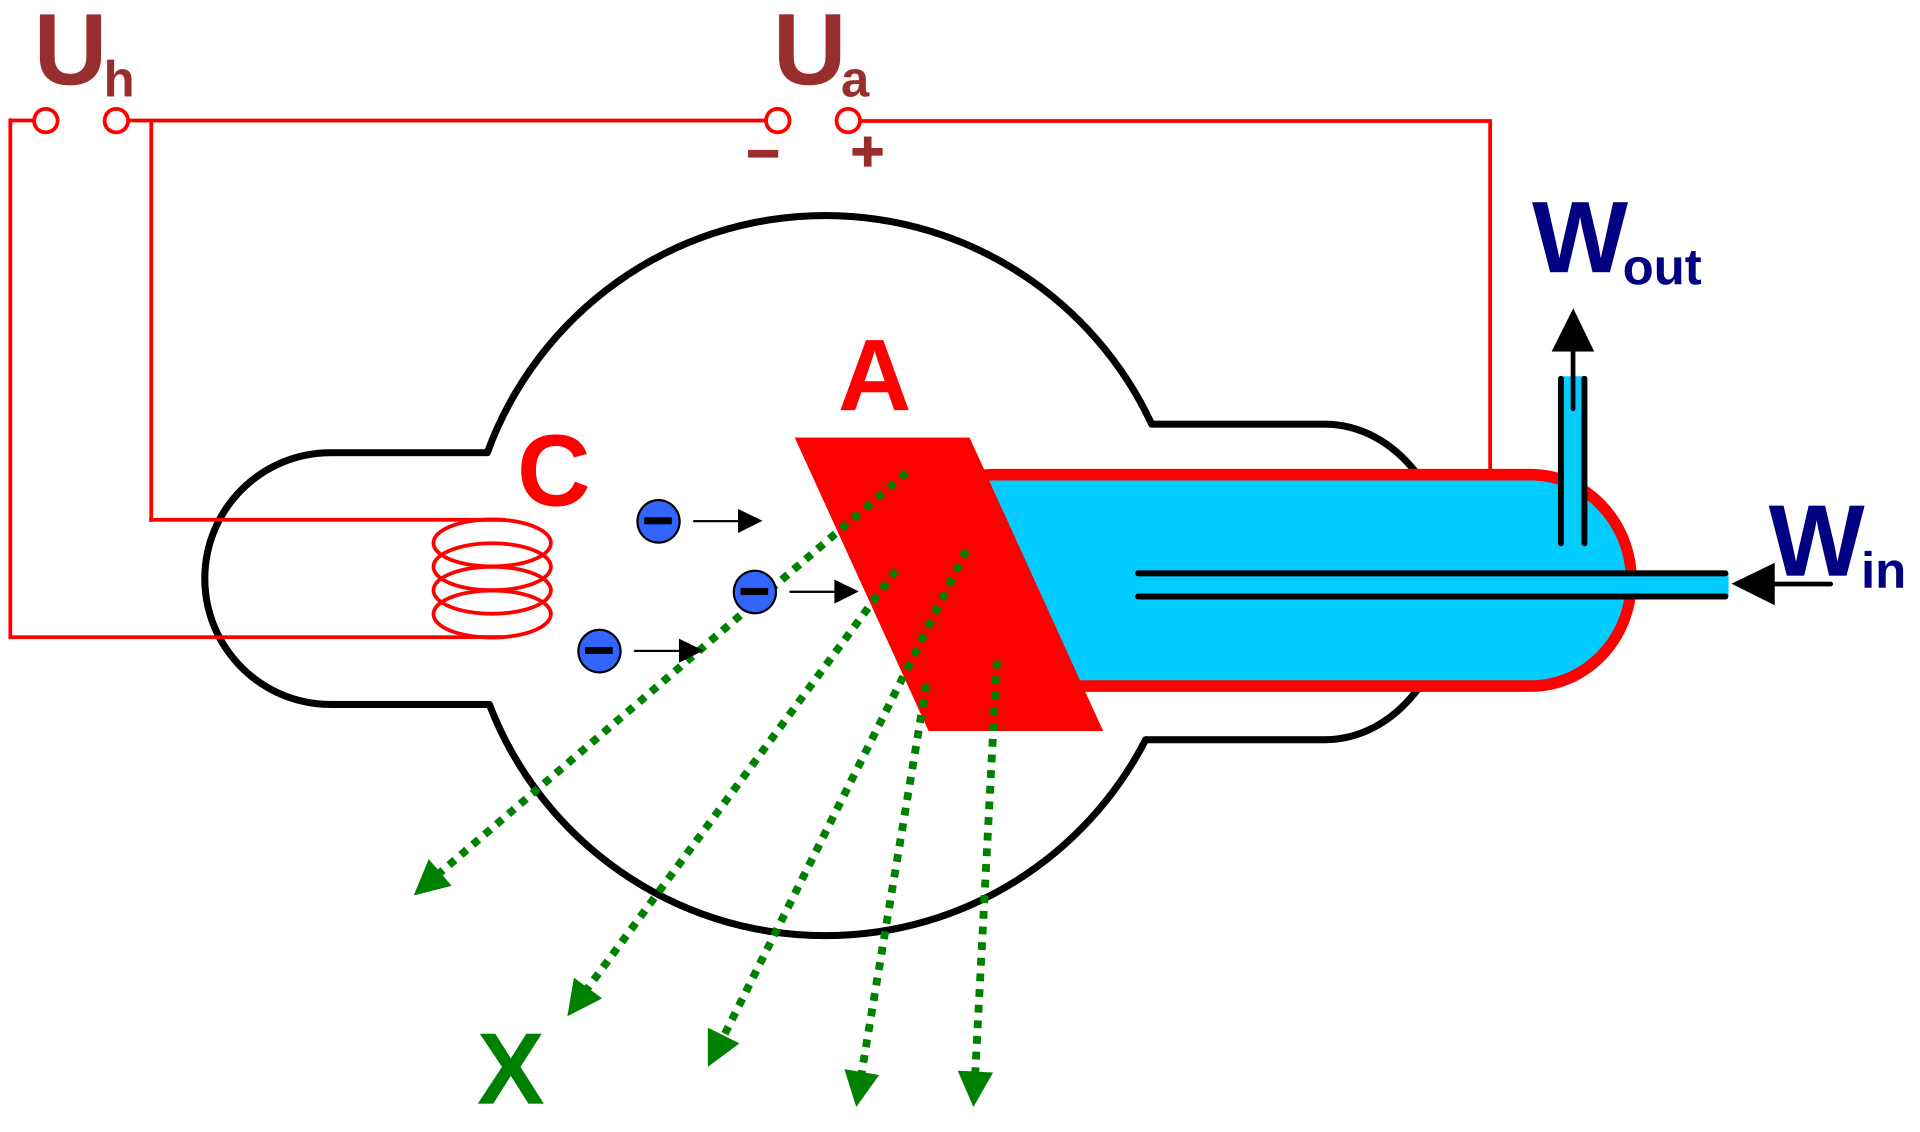
\includegraphics[width=15cm]{XRayTubeSketch}
\end{centering}
This is a sketch of a water-cooled X-Ray tube taken from Wikipedia. C is the Cathode and A is the Anode. The water cooling system won't be mentioned as it is not important in general.

We have a Potential $U_h$ which goes through the Cathode, heating it in the process. This process emits electrons through thermionic emission. 
The electrons are accelerated toward the Anode via the potential $U_a$, such that the Anode is positively charged, attracting the electrons. The Anode is made of metal, in our case tungsten.
The electrons knock out on-shell-electrons of the tungsten atoms, which leads to higher energy electrons falling into the holes left behind, producing X-Rays. Some electrons are also slowed by the Nucleuses themselves, producing Bremsstrahlung.
\section{Preparatory measurements}

We will be making measurements of the X-Rays liberated electrons over time, to see how an increased or decreased time affects the amount of liberated electrons. We will be measuring over 15, 30 and 45 seconds. We will keep the Area that we measure over, and the Intensity with which the electrons arrive at our area of measurement equal. We then expect a relation of
\begin{equation}
	Q = \int \text dt\int \text dA I(r_0) = tAI(r_0),\;\;\; Q \propto t
\end{equation}
Measurement are made with 1.52mm aluminium filter. The tray is 30cm away from the source\\
The X-Ray tube shall be set to $120$ kV an $10$ mA. Measurements are in nC.

\begin{center}
	\begin{tabular}{||c||c|c|c||}
	\hline
		 & $15s$ & $30s$ & $45s$\\
	\hline
		Measurements & 8.25 & 18.27 & 28.06 \\
		     	& 8.3 & 17.89 & 27.72 \\
			& 8.44 & 18.14 & 27.97\\
			& 8.31 & 18.04 & 27.51\\
			& 8.52 & 18.68 & 27.55\\
	\hline
		Average & 8.364 & 18.204 & 27.762\\
	\hline
		Average of Squared & 69.966 & 331.458 & 770.778\\
	\hline
		Standard Deviation & 0.097 & 0.269 & 0.222\\
	\hline
	\end{tabular}
\end{center}
with the average and standard deviation:
\begin{gather}
	\langle\mu\rangle = \frac{\sum_i^n x_i}{n},\;\;\;\;
	\sigma = \sqrt{\langle\mu^2\rangle - \langle\mu\rangle^2}
\end{gather}
In relation to the Average, the Standard deviation goes down with increasing time, signifying a more accurate measurement. We also notice that there is a linear increase with time. This linear increase signifies the charge that is picked up. We can read off a slope of 0.64$nC/s$.

\begin{centering}
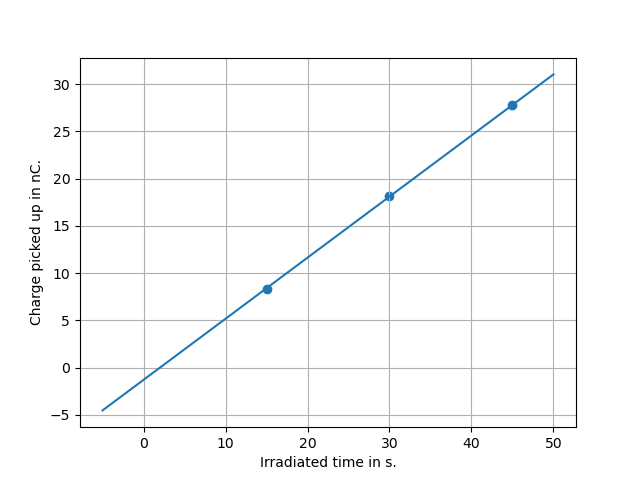
\includegraphics[width=15cm]{PrepMeasure}
\end{centering}
Such that we know that the Radiator sends off $0.64nC$ of charge every second. It is notable that despite being a perfect linear fit, the fit does not coincide with $f(t)=0$. This means that there is a loss of Charge in the first 10 seconds which is constant for all measured times. This can be explained by a short ramp up time that the X-Ray needs to go through first before operating at the desired Voltage and Amperage.
\section{Inverse square law}


Measuring the charge that is registered by a surface at different distances away from the source we can gather information about the relationship between Intensity of a field and distance away from the source. We assume that our findings will line up with the Inverse square law, so that $I(r) = I_0\frac{1}{r^2}$, where $r$ is the distance away from the center. This comes from the fact that we are measuring an Electromagnetic Wave, which is governed by $E = \frac{1}{4\pi\epsilon}\frac{Q}{r^2}$.\\

We will measure for 30s with the previous filter of 1.52mm, we will start at 30cm and end at 60cm in 5cm intervals. We use the previous measurement for 30cm.

\begin{center}
	\begin{tabular}{||c|c||}
		\hline
		Distance [cm] & Charge [-nC] \\
		30 & 18.00\\
		35 & 13.48\\
		40 & 10.36\\
		45 & 8.44\\
		50 & 6.91\\
		55 & 5.52\\
		60 & 4.74\\
		\hline
	\end{tabular}
\end{center}

Plotting the Charge against the inverse square of the distance should give a linear plot.

\begin{centering}
	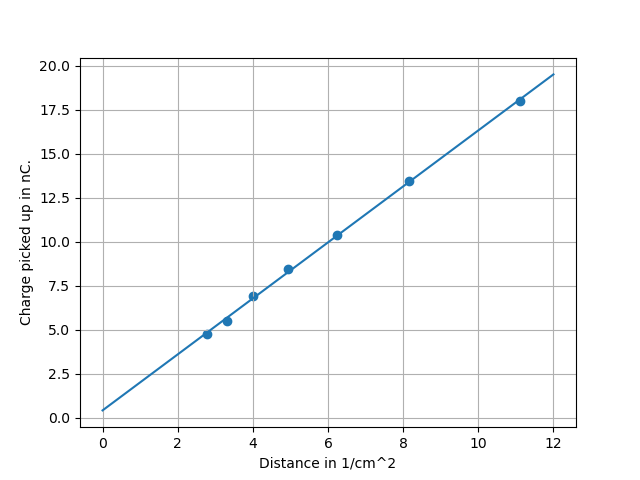
\includegraphics[width=15cm]{InvSquare}
\end{centering}
So it is clear that despite small deviations stemming from measurement Errors, the inverse square law is obeyed. I also plotted the datapoints against an inverse square function, and they line up.
\begin{centering}
	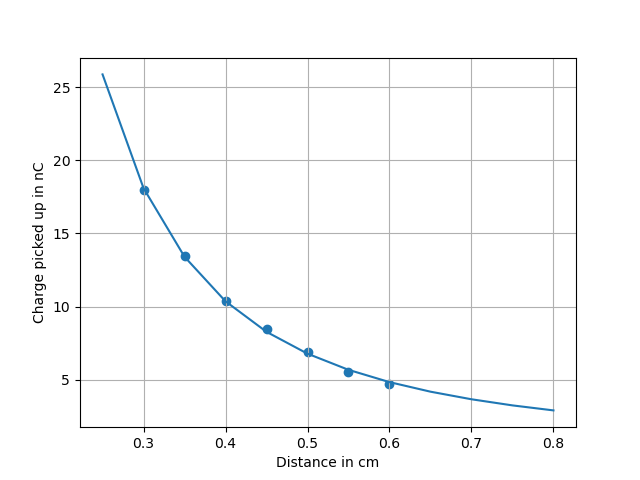
\includegraphics[width=15cm]{InvSquared2}
\end{centering}

This shows that, as we had previously expected, that X-Rays obey the inverse square law.




\section{Exponential photon attenuation}
The Photon attenuation law is a law that concerns the resulting intensity when photons travel through a Medium. Mathematically we state this as
\begin{equation}
	N_x = N_0 \exp(-\mu x)
\end{equation}
where $N_x$ is the amount of photons after interacting with the medium, and $N_0$ is the incoming amount of photons. $\mu$ is the linear attenuation coefficient, and represents how much Intensity is lost through the medium per distance, it has units $1/m$. $x$ is the distance that the photons travel through.

We can reduce this equation to a linear equation in x, so that we can determine the coefficient $\mu$ by using the relation
\begin{equation}
	\ln(N_x/N_0) = -\mu\cdot x
\end{equation}
So, we will use the logarithm of Intensity that is left and graph it against the length of the medium through which it travelled. The resulting linear fit will give us a coefficient $y = mx$ with $m=\mu$. We will pick $N_0$ such that the first measurement of $N_x = N_0$. This will result in a linear fit where we can ignore the coefficient $b$ in
\begin{equation}
	\ln(N_x/N_0) = -\mu\cdot x + b
\end{equation}
We will put the measuring device at 30cm
\begin{center}
\begin{tabular}{|c|c|}
\hline
	Material Width [mm] & Charge [-nC]\\
	\hline
1.52 &  18.00\\
2.02 &  16.14\\
2.52 &  14.54\\
3.02 &  13.11\\
4.02 &  11.05\\
\hline
\end{tabular}
\end{center}
Performing a linear fit gives us the plot:

\begin{centering}
	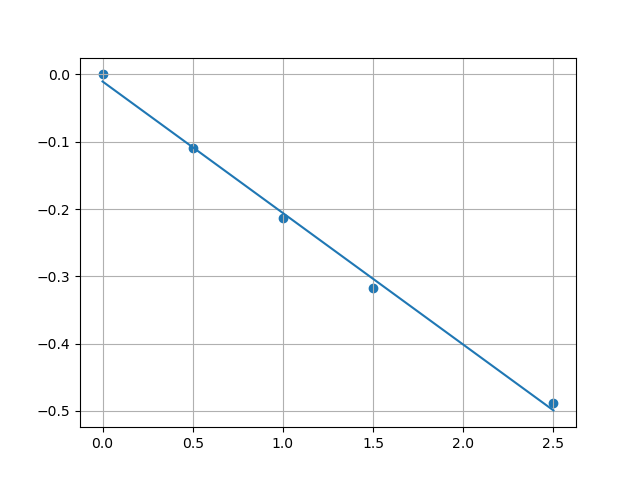
\includegraphics[width=15cm]{Attenuation Coeff}
\end{centering}

Which gives us an Attenuation Coefficient of $\mu = 0.195$.
\newpage
\section{Ionizations and radiation dose}

We define the Radiation dose.

\begin{equation}
	D = \frac{Q}{m}\left(\frac{W}{e}\right) = \frac{Q}{m}\cdot 34 J/C
\end{equation}
We use the Ideal gas law to calculate the mass of the Air inside the chamber.
\begin{gather}
	pV = nRT,\;\;\;\; \frac{pV}{RT} = n,\\
	\frac{pV}{RT}m_{Air,mol} = m
\end{gather}
Where we have $V=0.65cm^3$ and $m_{Air,mol} = 28.97 g/mol$. Inserting the usual Temperature and Pressure, $p= 101325 Pa$ and $T = 298K$ we can calculate the mass
\begin{equation}
	\frac{101325 Pa \cdot 0.00000065 m^3}{8.314 J/(mol K) \cdot 298K} \cdot 28.97 g/mol = 0.00077g
\end{equation}
and we have $1.6\cdot 10^{19}$ Air molecules in the chamber. We can now calculate the radiation dose after 45 seconds of Radiation, taking the measurement of $27.7nC$ from the previous experiment.
\begin{gather}
	\frac{27.7nC}{0.00077g}34 J/C = 1.22Sv
\end{gather}

We will calculate the ratio of ionized molecules after an exposure of $45s$. We assume that every molecule can only lose one electron, and therefore we must calculate how many electrons have a charge of $27.7nC$.
\begin{gather}
	\frac{27.7nC}{e} = \frac{27.7nC}{1.6022\cdot 10^{-10}nC} = 1.72\cdot 10^{11}
\end{gather}
We can see just from the order of magnitudes of the numbers, that the ionized molecule are a very small percentage of the total molecules. We calculate:
\begin{gather}
	\frac{1.72\cdot 10^{11}}{1.6\cdot 10^{19}} = 1.075\cdot 10^{-8} \approx 0.000001\%
\end{gather}
So about $0.000001\%$ of Air molecules were Ionized in those 45 seconds. 

\section{Conclusion}

We have learned different things about X-Rays. Firstly we learned that the Energy they give off is constant if we do not change the Voltage and Amperage of the X-Ray tube. We learned that they behave as Electromagnetic waves would, following the inverse square law. We also learned that Radiaton passes through material but gets weaker depending on the material, and with the thickness of the material. At last we have learned that Despite a large radiation dose (In our case $1.22Sv$) only a tiny percentage of air molecules are actually ionized in the end.
\end{document}

